%% dissertation.tex - PhD dissertation
%%
%% Copyright 2016 Jeffrey Finkelstein.
%%
%% This LaTeX markup document is made available under the terms of the Creative
%% Commons Attribution-ShareAlike 4.0 International License,
%% https://creativecommons.org/licenses/by-sa/4.0/.
\documentclass[draft]{article}

\usepackage{amsmath}
\usepackage{amssymb}
%% This must come before hyperref.
\usepackage{amsthm}
%% This is strongly recommended by biblatex.
\usepackage[english]{babel}
\usepackage[backend=biber]{biblatex}
\usepackage[T1]{fontenc}
%% This must come before csquotes.
\usepackage[utf8]{inputenc}
\usepackage{lmodern}
%% This is strongly recommended by biblatex.
\usepackage{csquotes}
%% This must come before hyperref.
\usepackage{thmtools}
%% This must come before complexity.
\usepackage{hyperref}
\usepackage{complexity}
\usepackage[firstpage]{draftwatermark}
\usepackage[final]{microtype}
\usepackage{textcomp}
\usepackage{tikz}

%% Set the amount by which certain characters protrude into the margins.
%%
%% \LoadMicrotypeFile{cmr}
%%
%%     This command forces the built-in protrusion settings for the Computer
%%     Modern Roman (cmr) font family to become available at this point, so
%%     that we can override these settings on the next line. Even though we are
%%     really using the Latin Modern Roman (lmr) fonts, microtype uses the cmr
%%     configuration file.
%%
%% \SetProtrusion
%%
%%     This instructs the microtype package that we are going to modify the
%%     protrusion settings.
%%
%% [load=lmr-T1]
%%
%%     Loads the Type 1 (T1) encoding of the lmr font family, thereby setting
%%     the default protrusion values for all the characters. This is only
%%     possible after the \LoadMicrotypeFile{cmr} command (microtype
%%     essentially considers lmr to be an alias for cmr).
%%
%% {encoding=T1, family=lmr}
%%
%%     Indicates that we are going to modify the protrusion values for the T1
%%     encoding of the lmr font family.
%%
%% \textquotedblright = {,1000} (and similar commands)
%%
%%     Force the character given by \textquotedblright to have default
%%     protrusion on the left margin (given by an empty string before the
%%     comma) and full protrusion (that is, protrusion value 1000) on the right
%%     margin.
\LoadMicrotypeFile{cmr}
\SetProtrusion
    [load=lmr-T1]
    {encoding=T1, family=lmr}
    {
      \textquotedblright = {,1000},
      \textquotedblleft = {1000,},
      {'} = {,1000},
      {,} = {,1000},
      {:} = {,1000},
      {;} = {,1000},
      {.} = {,1000}
    }

%% Set the ``work-in-progress'' watermark for the first page.
\SetWatermarkLightness{0.9}
\SetWatermarkText{Work-in-progress}
\SetWatermarkFontSize{3.5cm}

%% Set the title and author of the PDF file.
\hypersetup{pdftitle={PhD dissertation}, pdfauthor={Jeffrey Finkelstein}}

%% Declare the bibliography file.
\addbibresource{dissertation.bib}

%% Declare theorem-like environments.
\declaretheorem[numberwithin=section]{theorem}

%% Custom commands are declared here.
\newcommand{\email}[1]{\textlangle\href{mailto:#1}{\nolinkurl{#1}}\textrangle}
\newcommand{\todo}[1]{\textbf{TODO #1}}

\newcommand{\dash}{\textnormal{-}}

%% Redefine the footnote environment so it has no reference and no number.
\long\def\symbolfootnote#1{\begingroup%
\def\thefootnote{\fnsymbol{footnote}}\footnotetext{#1}\endgroup}

%% Define the author, title, and date for the document.
\author{Jeffrey~Finkelstein}
\title{Dissertation}

\begin{document}

\maketitle

\symbolfootnote{%
  Copyright 2016 Jeffrey~Finkelstein \email{jeffreyf@bu.edu}.

  This document is licensed under the Creative Commons Attribution-ShareAlike 4.0 International License, which is available at \mbox{\url{https://creativecommons.org/licenses/by-sa/4.0/}}.
  The \LaTeX{} markup that generated this document can be downloaded from its website at \mbox{\url{https://github.com/jfinkels/dissertation}}.
  The markup is distributed under the same license.
}

%% Document content goes here.
%
% Global components at each level must follow this structure.
%
% % Foreword %
%
% %% Context (anyone - why now?) %%
%
% What is the current situation, and why is the need so important?
%
%
% %% Need (readers - why you?) %%
%
% Why is this relevant to the reader, and why does something need to be done?
% (Also reference relevant existing work.)
%
%
% %% Task (author - why me?) %%
%
% What was undertaken to address the need?
%
%
% %% Object (document - why this document?) %%
%
% What does this document cover?
%
%
% % Summary %
%
% %% Findings (author - what?)
%
% What did the work reveal when performing the task?
%
%
% %% Conclusion (readers - so what?)
%
% What did the findings mean for the audience?
%
%
% %% Perspective (anyone - what now?)
%
% What should be done next?

\todo{Add quote from the Conclusions section of Buss and Goldsmith, ``Nondeterminism within P'': ``A fundamental question is whether there are problems \ldots''}

\begin{minipage}[t]{0.31\linewidth}
  \centering
  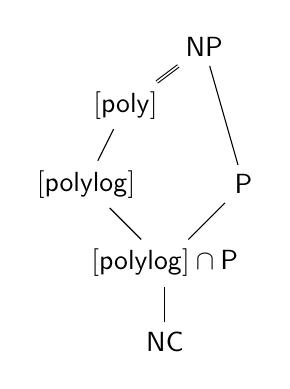
\begin{tikzpicture}
  \node at (0, 0) (nc) {$\NC$};
  \node at (0, 1) (both) {$\NNC[\polylog] \cap \P$};
  \node at (-1, 2) (nncpolylog) {$\NNC[\polylog]$};
  \node at (1, 2) (p) {$\P$};
  \node at (0.5, 3.75) (np) {$\NP$};
  \node at (-0.5, 3) (nnc) {$\NNC[\poly]$};

  \draw (nc) to (both);
  \draw (both) to (nncpolylog);
  \draw (both) to (p);
  \draw (p) to (np);
  \draw (nncpolylog) to (nnc);
  \draw[double] (nnc) to (np);
\end{tikzpicture}

\end{minipage}%
\begin{minipage}[t]{0.31\linewidth}
  \centering
  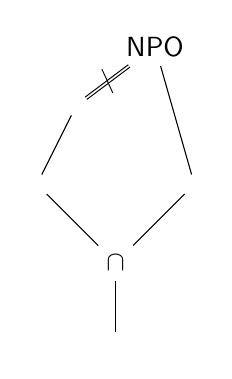
\begin{tikzpicture}
  \node at (0, 0) (nco) {$\NCO$};
  \node at (0, 1) (both) {$\ApxNCO \cap \PO$};
  \node at (-1, 2) (apxnco) {$\ApxNCO$};
  \node at (1, 2) (po) {$\PO$};
  \node at (0.5, 3.75) (npo) {$\NPO$};
  \node at (-0.5, 3) (nnco) {$\NNCO$};

  \draw (nco) to (both);
  \draw (both) to (apxnco);
  \draw (both) to (po);
  \draw (po) to (npo);
  \draw (apxnco) to (nnco);
  \draw[double] (nnco) -- (npo) node [rotate=45, midway] {\small$/$};
\end{tikzpicture}

\end{minipage}%
\begin{minipage}[t]{0.31\linewidth}
  \centering
  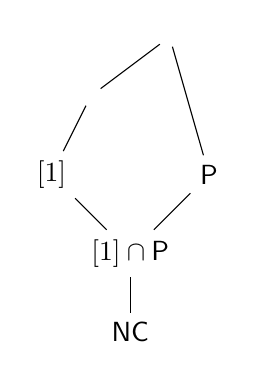
\begin{tikzpicture}
  \node at (0, 0) (fpnc) {$\para \NC$};
  \node at (0, 1) (both) {$\para \WNC[1] \cap \para \P$};
  \node at (-1, 2) (dontknow) {$\para \WNC[1]$};
  \node at (1, 2) (fpt) {$\para \P$};
  \node at (0.5, 3.75) (wp) {$\para \WP$};
  \node at (-0.5, 3) (wpp) {$\para \WNC$};

  \draw (fpnc) to (both);
  \draw (both) to (dontknow);
  \draw (both) to (fpt);
  \draw (fpt) to (wp);
  \draw (dontknow) to (wpp);
  \draw (wpp) to (wp);
\end{tikzpicture}

\end{minipage}

These inclusion diagrams shape how we approach all the problems in this paper.
Is there a $\P$-complete problem that is also
\begin{enumerate}
\item[(D1)] not in $\NNC[\polylog]$, unless $\NC = \P$?
\item[(D2)] in $\NNC[\polylog]$?
\item[(O1)] not in $\ApxNCO$, unless $\NC = \P$?
\item[(O2)] in $\ApxNCO$?
\item[(P1)] not in $\para \WNC$, unless $\NC = \P$?
\item[(P2)] not in $\para \NC$, unless $\NC = \P$?
\item[(P3)] in $\para \NC$?
\end{enumerate}

\section{Outline}

The referenced theorems correspond to the theorems in the respective papers.

\paragraph{Decision Problems.}
Completed:
\begin{enumerate}
\item $\NC = \PCP[O(\log \log n, O(1)]$ (Theorem~3.3).
\item $\NNC[\polylog] = \PCP[O(\log \log n), \polylog]$ (Corollary~3.2).
\item $\NP = \PCP[O(\log n), O(1)]$ (Theorem~3.4).
\item negative consequences $\PCP$ hierarchy collapses (Corollary~3.6) (\emph{relates to parameterized problems})
\item consequences of $\P = \PCP[O(\log \log n), \polylog]$ (Theorem~3.9).
\end{enumerate}
To-do:
\begin{enumerate}
\item Conjecture: inapproximability of High Degree Subgraph problem (Section~4) (\emph{relates to optimization problems}).
\end{enumerate}

\paragraph{Optimization problems.}

Completed:
\begin{enumerate}
\item $\NNCO$-complete problem (Theorem~3.3).
\item $\NPO$-complete problem (Corollary~3.4).
\item $\NNCO = \NPO \iff \NC = \P$ (Theorem~3.5).

\item $\PO$-complete problem (Theorems~3.8 and 3.9).
\item $(\PO \cap \NNCO)$-complete problem (Corollary~3.11).
\item $\PO \cap \NNCO = \PO \iff \NC = \P$ (Theorem~3.12).

\item $\PO \cap \NNCO$ is not closed under $\leq_m^{AP}$ reductions (Corollary~3.10).

\item Strictness of $\NNCO$ approximation hierarchy (Theorem~3.24).
\item Strictness of $\PO \cap \NNCO$ approximation hierarchy (Theorem 3.25).
\end{enumerate}
To-do:
\begin{enumerate}
\item Conjecture: $\ApxNCO$-complete problem (Section~3.3).
\item Conjecture: descriptive complexity characterization of $\ApxNCO$ (Section~4) (\emph{relates to parameterized problems}).
\item Conjecture: reduction preserving both verification complexity and approximability.
\end{enumerate}

\paragraph{Parameterized problems.}
Completed:
\begin{enumerate}
\item Circuit value problem is $\P$-complete but in $\para \AC^{0 \uparrow}$ (Theorems~3.3 and 3.5).
\item Nonuniform circuits for proving $\NC = \NNC[i(n) \log n] \implies \para \NC = \para \WNC$.
\item $\mathcal{O} \in \ENCAS \implies p \dash \mathcal{O} \in \para \NC$ (Theorem~3.18)
\item $\para \P$-complete problems (Section~4.2).
\item Definition of $\para \WNC[t]$?
\item $\para\NC = \para \WNC[t] \iff \Pi_t\LOGTIME[i(n) \log n] \subseteq \NC^d$, if it's correct (Section~6.4).
\end{enumerate}
To-do:
\begin{enumerate}
\item Change $\FPP$ to $\para \NC$ and $\WP[P]$ to $\para \WNC$.
\item Use depth $f(k) + \log^d n$ instead of $f(k) \log^d n$ depth; this will improve some of the depth bounds in some collapses (Theorem~5.8, Theorem~5.10, etc.).
\item Sideline the results for depth $g(k) \log^d n$ circuits instead of $f(k) + \log^d n$, since these correspond to the $\para \NC^{i\uparrow}$ classes.
\item Rename $\E[P]$ to $\para \EP$.
\item Add: related info from EST to section on $\para \P$-complete problems.
\item Add: the complete problem for $\para \WNC^1$ from \autocite{est15} into the proof of $\NC = \NNC[i(n) \log n] \implies \para \NC = \para \WNC$ (Section~5.3, Assumption~5.7, Theorem~5.8).
\item Add: theorem similar to Theorem~5.8 but concerning $\para \WL$ from \autocite{cm14}.
\item Add: $\para \WNC^d \subseteq \para \P \iff \W[\textsc{sat}] = \para \P$ from \autocite[Corollary~3.8]{est15} (Section~5.5).
\item Add: $p \dash \textsc{Group Rank}$ is a restriction of $p \dash \textsc{agen}$, and is in $\para \WL$, not known to be in any lower class (Theorem~5.3 and Section~6.2) (\emph{relates to decision problems}).
\item Remove: $p \dash \textsc{Group Rank}$ in $\para \WNC^1$: it is only in $\L$.
\item Conjecture: extend \autocite[Corollary~3.8]{est15} to $\para \WNC^d \subseteq \para \P$ implies $\W[\NC^d \textsc{sat}] = \para \P$?
\item Conjecture: show that collapses in the inclusion chain $\para \WNC^1$ through $\para \WP$ imply corresponding collapses in decision problems? This should follow from ``Describing parameterized complexity classes'' by Flum and Grohe (Section~5.6) (\emph{relates to decision problems}).
\item Conjecture: provide descriptive complexity characterizations of the $\para \W \mathcal{C}$ classes?
\item Conjecture: $\para \WNC^1[t] \subseteq \para \P$ if and only if a class between $\W[t] = \para \P$?
\end{enumerate}

%% Print the bibliography section here.
\printbibliography

\end{document}
